\documentclass{article}
\usepackage{amsfonts, amsthm, amsmath, amssymb, mathtools, ulem, mathrsfs, physics, esint, siunitx, tikz-cd}
\usepackage{pdfpages, fullpage, color, microtype, cancel, textcomp, markdown, hyperref, graphicx}
\usepackage{enumitem}
\graphicspath{{./images/}}
\usepackage[english]{babel}
\usepackage[autostyle, english=american]{csquotes}
\MakeOuterQuote{"}
\usepackage{xparse}
\usepackage{tikz}

% fonts
\def\mbb#1{\mathbb{#1}}
\def\mfk#1{\mathfrak{#1}}
\def\mbf#1{\mathbf{#1}}
\def\tbf#1{\textbf{#1}}

% common bold letters
\def\bP{\mbb{P}}
\def\bC{\mbb{C}}
\def\bH{\mbb{H}}
\def\bI{\mbb{I}}
\def\bR{\mbb{R}}
\def\bQ{\mbb{Q}}
\def\bZ{\mbb{Z}}
\def\bN{\mbb{N}}

% brackets
\newcommand{\br}[1]{\left(#1\right)}
\newcommand{\sbr}[1]{\left[#1\right]}
\newcommand{\brc}[1]{\left\{#1\right\}}
\newcommand{\lbr}[1]{\left\langle#1\right\rangle}

% matrices
\newcommand{\m}[2][b]{\begin{#1matrix}#2\end{#1matrix}}
\newcommand{\arr}[3][\sbr]{#1{\begin{array}{#2}#3\end{array}}}
\DeclareMathOperator{\Span}{span}

% greek
\newcommand{\e}{\epsilon}
\newcommand{\p}{\varphi}
\renewcommand{\t}{\theta}
\renewcommand{\l}{\lambda}
\renewcommand{\u}{\mu}
\renewcommand{\d}{\delta}

% misc
\NewDocumentCommand{\app}{O{x} O{\infty}}{\xrightarrow{#1\to#2}}
\newcommand{\sse}{\subseteq}
\renewcommand{\ss}{\subset}
\newcommand{\vn}{\varnothing}
\newcommand{\inv}{^{-1}}
\newcommand{\imp}{\implies}
\newcommand{\impleft}{\reflectbox{$\implies$}}
\renewcommand{\ip}[2]{\lbr{#1,#2}}
\renewcommand{\bar}{\overline}
\DeclareMathOperator{\cis}{cis}
\DeclareMathOperator{\Arg}{Arg}
\newcommand{\pf}{\tbf{Proof. }}

% title
\title{Scientific Computing HW 4}
\author{Ryan Chen}
%\date{\today}
\setlength{\parindent}{0pt}


\begin{document}
	
\maketitle



\begin{enumerate}
	
	
	
	\item We follow the notation of the lecture notes. Assume $A$ is $n\times n$ with distinct eigenvalues hence diagonalizable, with eigendecomposition
	\[A = R\Lambda R\inv\]
	Then the columns $r_j$ of $R$ are right eigenvectors, while the rows $l_k$ of $L:=R\inv$ are left eigenvectors. Moreover, $l_kr_j=0$ for $k\ne j$. Write $\dot r_j$ in the basis of $r_j$'s,
	\[\dot r_j = \sum_{l=1}^n m_{jl}r_l\]
	From the lecture notes,
	\[\dot Ar_j + A\dot r_j = \dot\l_jr_j + \l_r\dot r_j\]
	Left--multiply both sides by $l_k$ with $k\ne j$.
	\[l_k\dot Ar_j + \l_km_{jk} = \l_jm_{jk}
	\imp m_{jk} = \frac{l_k\dot Ar_j}{\l_j-\l_k}\]
	We can assume $m_{jj}=0$. Then
	\begin{align*}
		\Delta r_j &= \dot r_j\Delta t + O(\norm{\Delta A}^2) & \text{from lecture notes} \\
		&= \sum_{k\ne j} m_{jk}r_k\Delta t + O(\norm{\Delta A}^2) \\
		&= \sum_{k\ne j} \frac{l_k\dot Ar_j}{\l_j-\l_k}r_k\Delta t + O(\norm{\Delta A}^2) \\
		&= \sum_{k\ne j} \frac{l_k\Delta Ar_j}{\l_j-\l_k}r_k + O(\norm{\Delta A}^2) \\
	\end{align*}
	Then
	\begin{align*}
		\norm{\Delta r_j} &\le \sum_{k\ne j} \frac{\abs{l_k\Delta Ar_j}}{\abs{\l_j-\l_k}}\norm{r_k} + O(\norm{\Delta A}^2) \\
		&\le \norm{\Delta A}\norm{r_j}\sum_{k\ne j}\frac{\norm{l_k}\norm{r_k}}{|\l_j-\l_k|} + O(\norm{\Delta A}^2) \\
		&\le \norm{\Delta A}\kappa(R)\norm{r_j}\sum_{k\ne j}\frac{1}{|\l_j-\l_k|} + O(\norm{\Delta A}^2) & \norm{l_k}\norm{r_k} \le \kappa(R) \\
	\end{align*}
	Thus
	\[\kappa(r_j;A) = \lim_{\e\to0}\max_{\norm{\Delta A}=\e}\frac{\norm{\Delta r_j}\norm{A}}{\e\norm{r_j}}
	\le \norm{A}\kappa(R)\sum_{k\ne j}\frac{1}{|\l_j-\l_k|}\]
	We see that $\kappa(r_j;A)\gg1$ if $\kappa(R)\gg1$ or $\l_k\approx\l_j$ for some $k\ne j$.
	
	
	
	\pagebreak
	
	
	
	\item Before answering each part, we cite the following
	\[\grad(x^TAx) = (A+A^T)x,
	\quad \grad(x^Tx) = 2x\]
	We compute
	\[\grad Q(x) = \frac{(x^Tx)(A+A^T)x - (x^TAx)2x}{(x^Tx)^2}\]
	Thus
	\[\grad Q(x) = 0
	\iff (x^Tx)(A+A^T)x = 2(x^TAx)x
	\iff (A+A^T)x = \frac{2x^TAx}{x^Tx}x\]
	
	\begin{enumerate}
		
		
		
		
		\item Under the condition $A$ is symmetric, the above computation gives
		\[\grad Q(x) = 0
		\iff Ax = \frac{x^TAx}{x^Tx}x
		\iff \br{\frac{x^TAx}{x^Tx},x} \text{ is an eigenpair of $A$}\]
		
		
		
		\item If $A$ is asymmetric, the above calculation says $\grad Q(x)=0$ iff $\br{\frac{2x^TAx}{x^Tx},x}$ is an eigenpair of $A+A^T$.
		
		
		
		
	\end{enumerate}



	\pagebreak
	
	
	
	\item
	
	\begin{enumerate}
		
		
		
		\item Lemma: If $A$ is nonsingular and $(\l,v)$ is an eigenpair of $A$ then $(\l\inv,v)$ is an eigenpair of $A\inv$.
		
		Proof of lemma: From $A$ being nonsingular, $\l\ne0$. Then
		\[Av = \l v
		\imp v = \l A\inv v
		\imp A\inv v = \l\inv v \qed\]
		
		Since $\u$ is not an eigenvalue of $A$, we know $A-\u I$ is nonsingular. Then
		\[(A-\u I)v = Av - \u Iv
		= \l v - \u v
		= (\l-\u)v\]
		hence $((\l-\u),v)$ is an eigenpair of $A-\u I$. By the lemma, $((\l-\u)\inv,v)$ is an eigenpair of $(A-\u I)\inv$.
		
		
		
		\item We assume $A$ is symmetric with distinct eigenvalues, so we can pick orthonormal eigenvectors $v_i$. First write
		\[\kappa((A-\u I)\inv,v) = \norm{(A-\u I)\inv}\frac{\norm{v}}{\norm{(A-\u I)\inv v}}\]
		Now we calculate each RHS factor. By construction, $\norm{v}=1$.
		
		Since $A$ has eigenpairs $(\l_i,v_i)$, by part (a), $(A-\u I)\inv$ has eigenpairs $((\l_i-\u)\inv,v_i)$. From $\mu\approx\l_1$ and $A$ having distinct eigenvalues, the eigenvalue of $(A-\u I)\inv$ with largest absolute value is $(\l_1-\u)\inv$, hence $\norm{(A-\u I)\inv}=\abs{\l_1-\u}\inv$.
		
		Since $(A-\u I)\inv$ has eigenpairs $((\l_i-\u)\inv,v_i)$,
		\[(A-\u I)\inv v = \sbr{1-\sum_{i=2}^n\d_i^2}^{1/2}\br{\l_1-\u}\inv v_1 + \sum_{i=2}^n\d_i\br{\l_i-\u}\inv v_i\]
		Thus
		\begin{align*}
			\norm{(A-\u I)\inv v} &= \brc{\sbr{1-\sum_{i=2}^n\d_i^2}\br{\l_1-\u}^{-2} + \sum_{i=2}^n\d_i^2\br{\l_i-\u}^{-2}}^{1/2} & \text{$v_i$'s are orthonormal} \\
			&= \brc{\br{\l_1-\u}^{-2} - \br{\l_1-\u}^{-2}\sum_{i=2}^n\d_i^2 + \sum_{i=2}^n\d_i^2\br{\l_i-\u}^{-2}}^{1/2} \\
			&= \brc{\br{\l_1-\u}^{-2} - \sum_{i=2}^n \d_i^2\sbr{\br{\l_1-\u}^{-2} - \br{\l_i-\u}^{-2}}}^{1/2}
		\end{align*}
	
		Putting together the calculations,
		\begin{align*}
			\kappa((A-\u I)\inv,v) &= \br{\br{\l_1-\u}^2}^{-1/2}\brc{\br{\l_1-\u}^{-2} - \sum_{i=2}^n \d_i^2\sbr{\br{\l_1-\u}^{-2} - \br{\l_i-\u}^{-2}}}^{1/2} \\
			&= \brc{1 - \sum_{i=2}^n \d_i^2\sbr{1 - \br{\frac{\l_1-\u}{\l_i-\u}}^2}}^{-1/2} \\
			&\approx \brc{1 - \sum_{i=2}^n \d_i^2}^{-1/2} & \u\approx\l_1
		\end{align*}
		
		
		
		\item Code: \url{https://github.com/RokettoJanpu/scientific-computing-1-redux/blob/main/hw4.ipynb}
		
		\begin{center}
			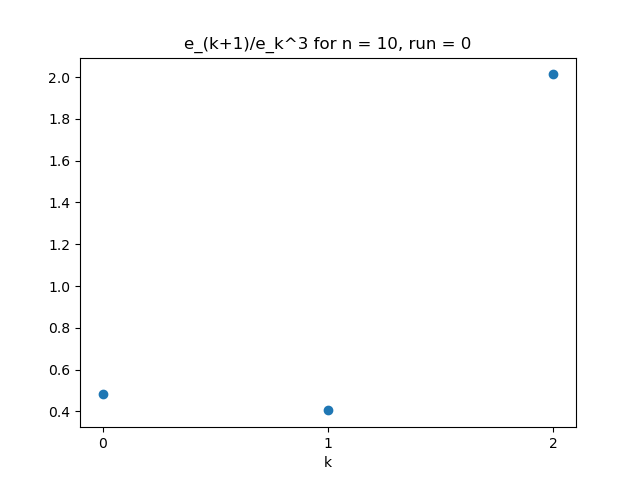
\includegraphics[scale=.4]{hw4 err n = 10 run = 0}
			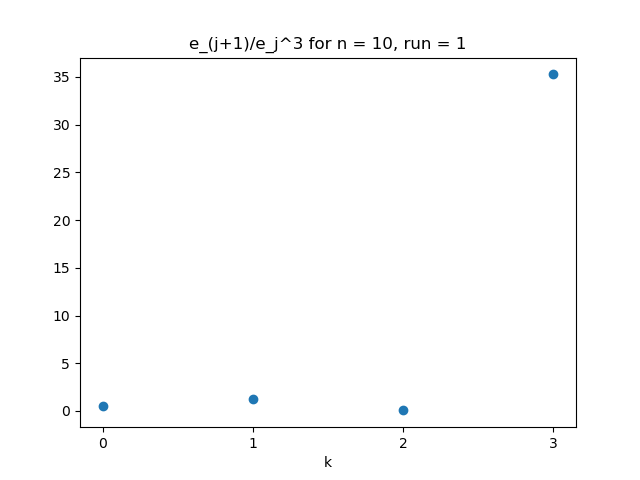
\includegraphics[scale=.4]{hw4 err n = 10 run = 1}
			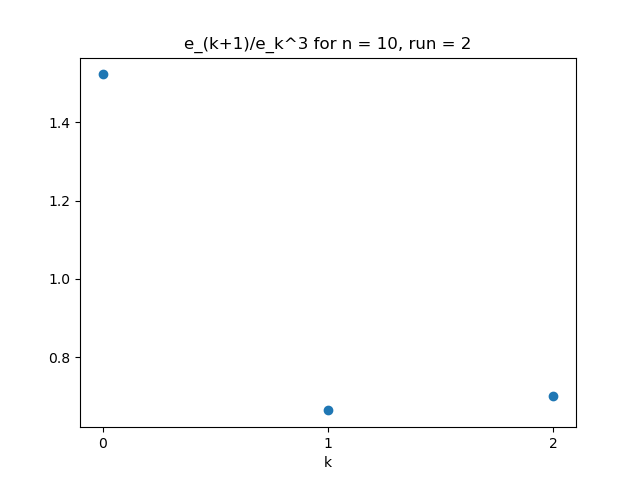
\includegraphics[scale=.4]{hw4 err n = 10 run = 2}
			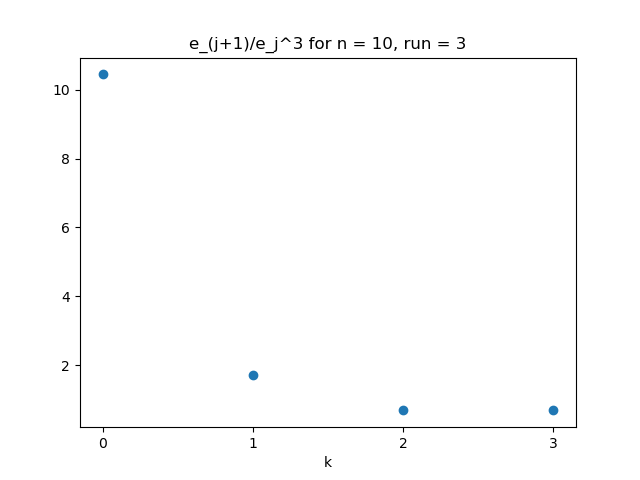
\includegraphics[scale=.4]{hw4 err n = 10 run = 3}
			
			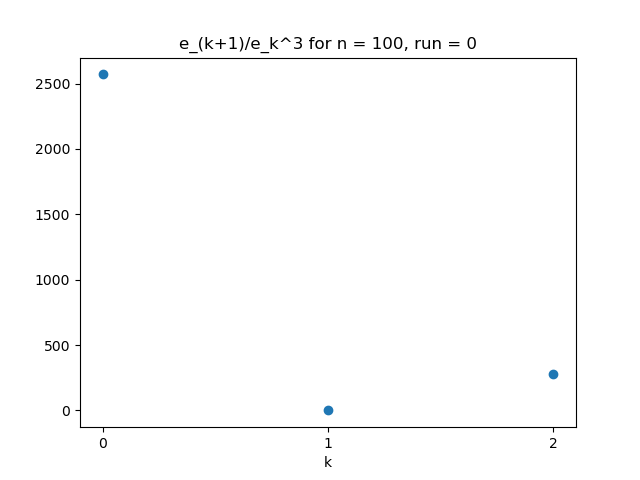
\includegraphics[scale=.4]{hw4 err n = 100 run = 0}
			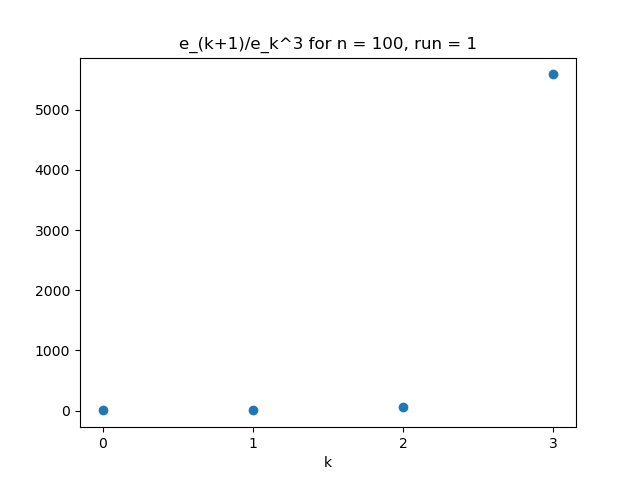
\includegraphics[scale=.4]{hw4 err n = 100 run = 1}
			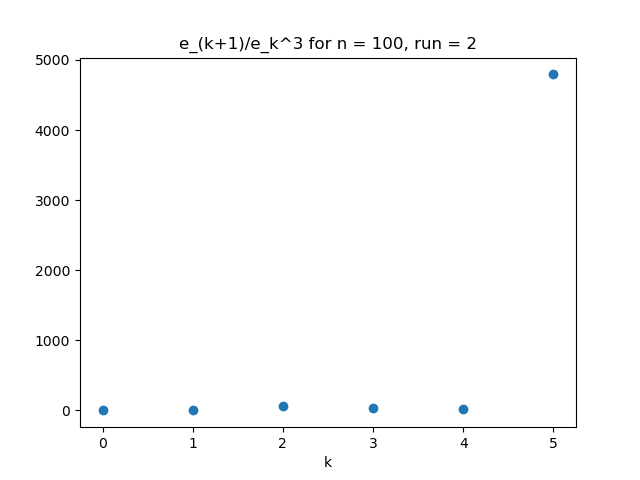
\includegraphics[scale=.4]{hw4 err n = 100 run = 2}
			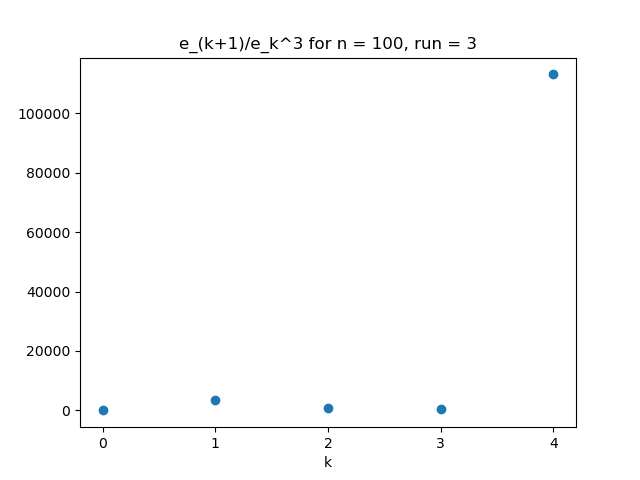
\includegraphics[scale=.4]{hw4 err n = 100 run = 3}
			
			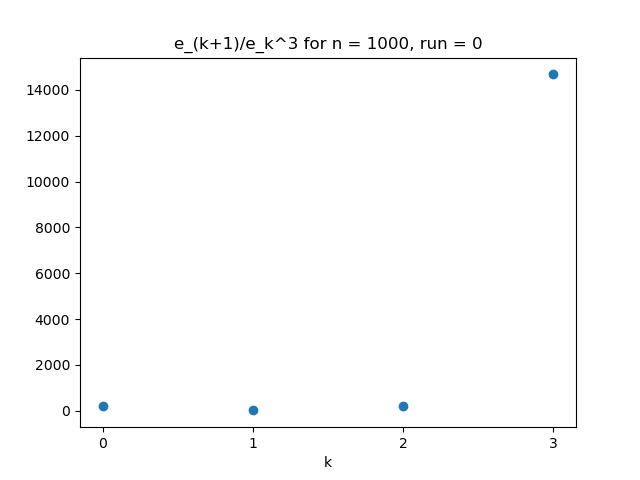
\includegraphics[scale=.4]{hw4 err n = 1000 run = 0}
			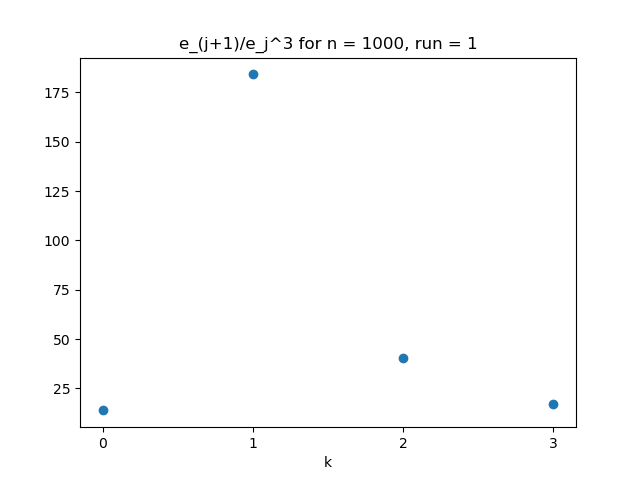
\includegraphics[scale=.4]{hw4 err n = 1000 run = 1}
			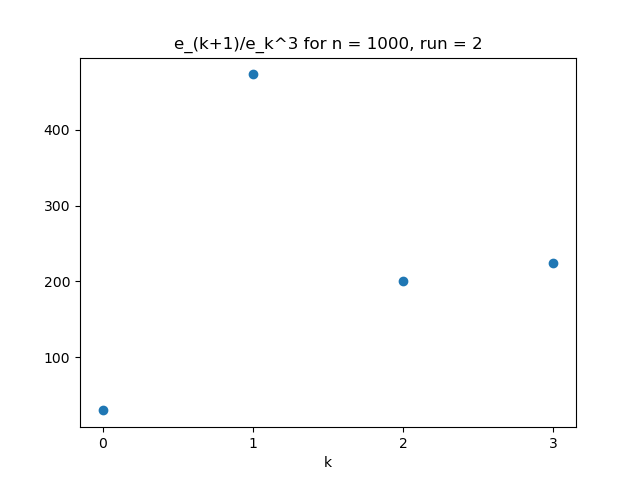
\includegraphics[scale=.4]{hw4 err n = 1000 run = 2}
			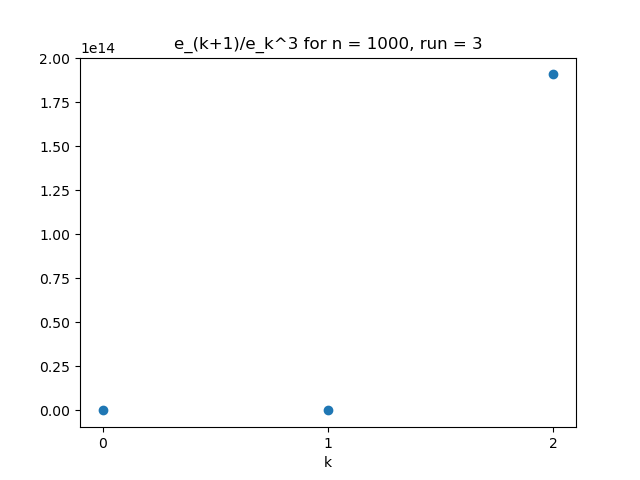
\includegraphics[scale=.4]{hw4 err n = 1000 run = 3}
		\end{center}
		Indeed, we do not have enough iterates to observe an eventual "leveling out" of the sequence $\frac{e_{j+1}}{e_j^3}$.
		
		
		
		
	\end{enumerate}
	
	
	
\end{enumerate}
	
	
\end{document}